\documentclass[11pt]{extarticle}
\usepackage[a4paper, total={6in, 8.5in}, top=1in, bottom=1in, left=1in, right=1in]{geometry}

\usepackage{mathtools}
\usepackage{graphicx}
\usepackage{amssymb}
\usepackage{amsmath}
\usepackage{pythonhighlight}
\usepackage{pdfpages}
\usepackage[T1]{fontenc}
\usepackage[utf8]{inputenc}
\usepackage{fancyhdr}
\usepackage{pythonhighlight}
\usepackage{changepage}
\usepackage{slashbox}
\usepackage{floatrow}
\usepackage{listings}
\usepackage[hidelinks]{hyperref}
\usepackage{fontawesome}
\usepackage{caption}
\usepackage{subcaption}
\usepackage{color} %red, green, blue, yellow, cyan, magenta, black, white
\definecolor{mygreen}{RGB}{28,172,0} % color values Red, Green, Blue
\definecolor{mylilas}{RGB}{170,55,241}


\floatsetup[table]{capposition=top}

\sloppy
\definecolor{lightgray}{gray}{0.5}
\setlength{\parindent}{0pt}
\setlength{\headheight}{14pt}

\renewcommand{\headrulewidth}{.4mm} % header line width
\newcommand{\norm}[1]{\left\lVert#1\right\rVert}

\pagestyle{fancy}
\fancyhf{}
\fancyhfoffset[L]{-1cm} % left extra length
\fancyhfoffset[R]{-1cm} % right extra length
\rhead{\bfseries Kutay U\u{g}urlu 2232841}
\lhead{EE583 Homework 6}
\rfoot{}

\DeclarePairedDelimiter\ceil{\lceil}{\rceil}
\DeclarePairedDelimiter\floor{\lfloor}{\rfloor}

\author{Kutay U\u{g}urlu 2232841}

\begin{document}
    
\lstset{language=Matlab,%
    %basicstyle=\color{red},
    breaklines=true,%
    morekeywords={matlab2tikz},
    keywordstyle=\color{blue},%
    morekeywords=[2]{1}, keywordstyle=[2]{\color{black}},
    identifierstyle=\color{black},%
    stringstyle=\color{mylilas},
    commentstyle=\color{mygreen},%
    showstringspaces=false,%without this there will be a symbol in the places where there is a space
    numbers=left,%
    numberstyle={\tiny \color{black}},% size of the numbers
    numbersep=9pt, % this defines how far the numbers are from the text
    emph=[1]{for,end,break},emphstyle=[1]\color{red}, %some words to emphasise
    %emph=[2]{word1,word2}, emphstyle=[2]{style},    
}

\fancyfoot[C]{\thepage}

\title{\LARGE \LARGE EE583 Pattern Recognition HW6}

\maketitle{\LARGE}

\pagebreak


\begin{figure}[h]
    \centering
    \begin{subfigure}[b]{0.45\textwidth}
        \centering
        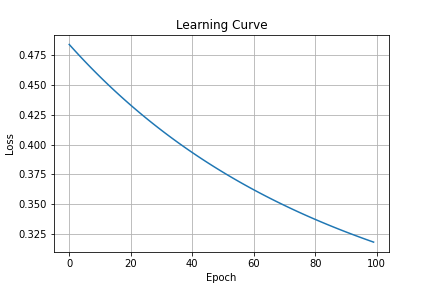
\includegraphics[width=\textwidth]{Q1.png}
        \caption{Q1 Learning Curve}
        \label{subfig:1a}
    \end{subfigure}
    \begin{subfigure}[b]{0.45\linewidth}
        \centering
        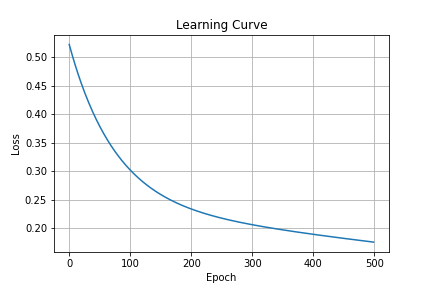
\includegraphics[width=\textwidth]{Q2.png}
        \caption{Q2 Learning curve}
        \label{subfig:1b}
    \end{subfigure}
    \caption{Q1}
\label{fig:Q1}
\end{figure}



\end{document}